\section{Introduction}
% Main goal: Argue for SC, and \xQ. Present \xQ{} and justify decisions. Demonstrate the performance on `realistic simulations'.

Thanks to advances in AI and machine learning, unmanned autonomous physical systems (APS) are poised to tackle complex decision making problems for high-consequence applications, such as wilderness search and rescue, transportation, agriculture, remote science, and space exploration. 
%Unlike low-level automation for assembly lines, cruise control, thermostats, etc., 
APS must be self-sufficient and make self-guided decisions about complex problems delegated by users. Hence, APS that are taskable---able to translate high-level commands into suitable processes for sensing, learning, reasoning, communicating, and acting --must also be cognizant and knowledge-rich--capable of reasoning about the capabilities and limitations of their own processes, anticipating possible failures, and able to recognize when they are operating incorrectly \cite{david2016defense}. %to adapt accordingly. %To ensure long-term robustness and resilience for minimally supervised operations, APS behaviors must be predictable, understandable, and explainable. %to human users/stakeholders. %, who in many cases can also provide collaborative high-level assistance or supervisory directives in difficult situations. 

This work is motivated by the need to develop new computational strategies for assessing when an APS reaches its \emph{competency boundaries}. If computed and communicated correctly, such assessments can provide users with clearer predictions of APS behavior and understanding of actual APS capabilities. This can not only allow APS to take initiatives to stay within its competency boundary in untested situations, but also provide users/stakeholders with assurances that allow them to properly calibrate trust in (and hence make proper use of) intelligent APS \cite{Israelsen2018-es}. 

These properties are especially important for APS that must rely heavily on non-deterministic algorithms for decision-making under uncertainty, i.e. to efficiently make approximate inferences with imperfect models, learn from limited data, and execute potentially risky actions with limited information. 
%From self-driving cars and unmanned aircraft on Earth to planetary rovers in space \cite{}, and from networked smart devices in the home to smart building systems \cite{}, such APS are now becoming a pervasive part of everyday reality. 
%Crucially, these systems require interaction among several different algorithmic components to support intelligent APS capabilities (for sensing, perception, planning, control, communication, etc.). 
%Algorithms for these capabilities are often studied in isolation, but not together... 
%\nisar{but not much work has been done in terms of holistically looking at APS operating under uncertainty -- expand on this in background...} 
Whereas most relevant and recent work on algorithmic introspection and meta-reasoning to date has focused on outcome-based analyses for  AI/learning agents with narrow well-defined tasks,
%such techniques are typically best suited to APS with relatively narrow well-defined capabilities and few computational resource constraints. Since many current and future APS must operate in open-ended task settings in physical environments with significant limitations (due to constrained platform size, weight, power, etc.), the interpretation of `favorable/unfavorable' outcomes can shift in subtle yet significant ways as a function of APS design and task context. To cope with broader classes of APS, %(i.e. engineered sum of interconnected algorithmic and physical parts), 
holistic process-based techniques for algorithmic competency boundary self-assessment are needed to accommodate broader classes of APS operating in complex, dynamic and uncertain real-world settings -- whose computational models and approximations are expected to break down in less obvious/foreknown ways. %\nisar{meh?}

This paper presents and builds on a recently developed algorithmic framework for computing and evaluating self-assessments in APS that leads to shorthand metrics of \emph{machine self-confidence}. Self-confidence is defined as an APS' perceived ability to achieve assigned goals after accounting for uncertainties in its knowledge of the world, its own state, and its own reasoning and execution abilities \cite{Aitken2016-cv, Aitken2016-fb, Sweet2016-tz}. 
Algorithmic computation of self-confidence is strongly linked to model-based assessments of probabilities pertaining to task outcomes and completion---but crucially goes further to provide insight into how well an APS's processes for decision-making, learning, perception, etc. are matched to intended tasks \cite{Hutchins2015-if}. 
We argue that the short-hand insight provided by self-confidence assessments can serve as a transparent and decomposable/traceable feedback signal to anticipate degraded, nominal, or enhanced APS performance, %adapt autonomous behavior, 
and thereby can be used to calibrate user trust in APS for uncertain task settings. 

The main contributions of this paper include: 1) A formal definition of `solver-quality' which is one of several factors that make up `self-confidence'. Herein, solver-quality is presented as a metric for assessing how competent an MDP solver is for a given task. 2) Solver-quality is then derived borrowing inspiration from empirical hardness models (EHMs \cite{Leyton-Brown2009-yr}. 3) Solver-quality is then evaluated using numerical experiments. The paper is organized as follows: In Section~\ref{sec:background} we further explore motivations and background for self-confidence, including concepts like trust between humans and autonomous systems, and a useful example application. In Section~\ref{sec:self-confidence} Factorized Machine Self-Confidence (\famsec) is introduced and a framework outlined. At the end of Section~\ref{sec:self-confidence} we turn our attention to one of the \famsec{} factors, `Solver Quality', and outline specific challenges and desiderata in the context of the broadly useful family of Markov Decision Process (MDP)-based planners. A learning-based technique for computing solver quality factors in MDP-family planners is then derived in Section~\ref{sec:methodology}. In Section~\ref{sec:results} we present results from numerical experiments for an unmanned autonomous vehicle navigation problem. Finally we present conclusions in Section~\ref{sec:conclusions}.

\section{Background and Related Work} \label{sec:background}
This section reviews several key concepts and related works which set the stage for our proposed computational machine self-confidence framework. To make the concepts discussed throughout the paper concrete and provide an accessible proof-of-concept testbed in later sections, we also describe a motivating APS application example inspired by ongoing research in unmanned robotic systems.  

\subsection{Autonomous Systems and User Trust}
An APS is generally any physical agent comprised of a machine controlled by some form of software-based autonomy. Autonomy defines the ability of the system to perform a complex set of tasks with little/no human supervisory intervention for extended periods of time. This generally means that an APS has at least one or more of the capabilities of an artificially intelligent physical agent, i.e. reasoning, knowledge representation, planning, learning, perception, motion/manipulation, and/or communication \cite{Israelsen2018-es}. 
Despite many popular myths and misconceptions, an APS always interacts with a human user in some way \cite{Bradshaw2013-ck}. 
That is, the aforementioned capabilities are the means by which an APS achieves some \emph{intended} degree of self-sufficiency and self-directedness for tasks that are \emph{delegated} by a user in order to meet an `intent frame' (desired set of goals, plans, constraints, stipulations, and/or value statements) \cite{Miller2014-av}. `Transparency' in this context thus shifts primary concern away from details of how exactly an APS accomplishes a task, towards knowing whether an autonomous system can/cannot execute the task per the user's intent frame. 
In cases where users must re-examine delegated tasks, the ability to interrogate an APS for details related to how tasks would be executed or why tasks can/cannot be completed become an important follow-on consideration for transparency (i.e. on a need to know `drill-down' basis). 
%%\nisar{hook to `drill down' req: user in high-consequence situation would want to know why/why not...and ask more questions as needed or as time/context permits... }

This view naturally sets up several questions related to user trust in autonomous systems. Trust defines a user's willingness and security in depending on an APS to carry out a delegated set of tasks, having taken into consideration its characteristics and capabilities. 
We focus here on the problem of how an APS can be designed to actively assist users in appropriately calibrating their trust in the APS. As surveyed in \cite{Israelsen2018-es}, several broad classes of \emph{algorithmic assurances} for APS have been developed, where an assurance is defined as any property or behavior that can serve to increase or decrease a user's trust. 
Good assurances are challenging to develop because they must allow users to gain better insight and understanding of APS behaviors for effectively managing operations, without undermining autonomous operations or burdening users in the process. 
Many assurance strategies, such as value alignment \cite{Dragan2014-gu} (where an APS adapts its behavioral objectives with a user's intent frame via interactive learning) and interpretable reasoning \cite{Ruping2006-xj} (where algorithmic capabilities for planning, learning, reasoning, etc. are made accessible and easy to understand for non-expert users) put the onus on the APS (and designers) to integrate naturally transparent trust-calibrating behaviors into core system functionality. 
Other strategies, such as those based on post hoc explanation for learning and reasoning systems \cite{Lacave2004-gq, Ribeiro2016-uc} and data visualization \cite{Sacha2017-hf}, require users to render their own judgments via processing of information provided by the APS (possibly in response to specific user queries). 
Indeed, while the full range of assurance design strategies for APS have much in common with techniques for ensuring transparency and accountability for more general AI and learning systems, assurances based on self-monitoring offer an especially promising path for APS competency assessment. 

\subsection{Self-Monitoring and Self-Confidence}
State of the art machine learning and statistical AI methods have ushered in major improvements to APS capabilities in recent years. 
Yet, as these methods and capabilities continue to improve and find new high-consequence applications, resulting APS implementations are also becoming more complex, opaque and difficult for users (as well as designers and certifying authorities) to fully comprehend. 
In particular, for sophisticated APS characterized by uncertainty-based reasoning and data-driven learning, it can become extremely difficult to make precise predictions about APS behavior and performance limits in noisy, untested, and `out of scope' task conditions with any degree of certainty. Formal verification and validation tools could be used to tackle these issues at design time, but do not provide assurances that can be readily conveyed to or understood by (non-expert) users at run-time. 
It can thus be argued that the task of assessing APS competency at run-time is in general so complex and burdensome that it should also be delegated to the APS itself. 

This leads to consideration of algorithmic self-monitoring methods, e.g. for introspective reasoning/learning \cite{Huang2017-zt}, fault diagnosis and computational meta-reasoning/meta-learning \cite{grant2018recasting}. 
While promising for a wide variety of applications, these methods depend heavily on task outcome and performance assessments, and often require data intensive evaluations. 
As such, these methods are often best-suited to APS with narrow, well-defined, capabilities and few computational resource constraints. 
However, many current and future APS must operate in open-ended task settings in physical environments with significant computational limitations (due to constrained platform size, weight, power, etc.). 
The interpretation of `favorable vs. unfavorable' task outcomes can also shift in subtle yet significant ways that may not be obvious to non-expert users, i.e. depending on the interactions of designed APS capabilities and task context (all of which may also change drastically over the course of a given operational instance). 

%\nisar{...makes it difficult for non-expert users to trace and drill down into and understand assessments... } 
%\nisar{TODO: briefly talk about other background things related to transparency for introspection, Dragan's critical states, meta-RL, meta-cog architectures, etc.; ... what are the drawbacks/limitations in context of autonomous systems? what moves us towards something different like self-confidence? key idea: these are largely outcome based and driven by achievement of robustness/resilience for task performance, as opposed to process-based and do not provide clear assessment/ability to quantify/qualify/communicate what APS actually can or cannot accomplish...taking meta RL as example: system will keep trying to do its best to learn... for critical state MDP: presumes that solver/models/reward functions used to come up with solution are in fact appropriate and that capabilities/scope given to system is in fact appropriate (solution/implementation of APS is not placed into context)}

%\nisar{something here to get into the idea of APS being different but not totally unrelated to ML/AI (e.g. consequences of failure might be loss of APS or damage/irreparable loss to surroundings, as well as dynamic settings...) --  (licensing argument, i.e. we don't certify humans, but do put them through a process-based licensing approach? basically: a big question/central tension here is: how to monitor/supervise APS within competency limits without undercutting very point of autonomy itself? )}

These limitations motivate consideration of \emph{process-based assessment} techniques that allow APS to more generally self-qualify their capabilities for a particular task by evaluating and reporting their associated degree of `self-trust' or \emph{self-confidence}. 
As evidenced by recent work in neurocomputational modeling of decision-making for visual-motor tasks,
self-confidence reporting in humans generally requires second-order reasoning about uncertainties associated with particular task outcomes, i.e. assessments of `uncertainties in uncertainty' as well as of one's own reasoning processes \cite{Adler2016-oi}.  This resonates with the machine self-confidence concept put forth by \cite{Hutchins2015-if}, who proposed using human expert evaluations of specific APS capabilities to manually encode where and when these may break down in particular tasking situations. 
Several formal definitions and techniques for allowing APS to automatically compute their own machine self-confidence scores in the context of different tasks and capability assessments have been proposed recently.
For instance, Kuter and Miller \cite{Kuter2015-qh} proposed to evaluate \emph{plan stability} for systems that rely on hierarchical task planning algorithms, using formal counter-planning methods to determine threatening contingencies for a given plan and plan repair techniques in order to assess the adaptability of that plan to circumvent those contingencies. 
This relies heavily on fixed knowledge bases and ontologies, and so only supports assessments for well-understood environments, tasks, systems, and contexts. 
These and other approaches are reviewed in \cite{Sweet2016-tz}, as well as in \cite{Israelsen2018-es} in the context of algorithmic interactions for human-autonomous system trust relationships. %, where self-confidence is identified as an explicit assurance in a human-autonomy trust relationship. 
%According to \cite{} the four views on self-confidence are the \textit{anthropomorphic view}, the \textit{uncertainty view}, the \textit{experiential view}, and the \textit{stability view}. The anthropomorphic view defines self-confidence to be similar to how humans express self-confidence, while the experiential view expresses self-confidence based on past experience. The uncertainty view simply defines self-confidence to be the probability of success or failure, and the stability view defines self-confidence to be the sensitivity of the probability of success to uncertainty. All of these views seem to reflect different parts of a more general concept: understanding an autonomous system's ability to do a specific task. 
For the sake of brevity, we restrict attention to the definition of self-confidence used in this work: \textbf{An agent's perceived ability to achieve assigned goals (within a defined region of autonomous behavior) after accounting for (1) uncertainties in its knowledge of the world, (2) uncertainties of its own state, and (3) uncertainties about its reasoning process and execution abilities.}

%\hlr{...also consider other self-confidence ideas/approaches (e.g. four different approaches considered in InfoTech paper) and algorithms (e.g. Ugur's plan robustness idea, surprise index, perception robustness/statistical residuals test)... one limitation of algs: only limited to specific segments or types of reasoning, rather than looking at interconnected processes holistically for autonomous *systems* }

\subsection{MDP-based Planning and Learning}
The diversity of factors that influence APS self-confidence requires a rich modeling approach for algorithmic assessment. We will therefore establish algorithmic realizations of self-confidence assessments by initially studying APS capabilities that can be defined or modeled via Markov decision processes (MDPs). MDPs are composed of finite states and actions that partially resolve the nondeterminism in the state transitions by deciding from what probability distribution $p(\cdot)$ the next state will be sampled. The co-existence of nondeterministic and stochastic choices in MDPs are expressive enough to account for a range of uncertainties including adversarial environmental factors and inaccuracies in execution. %%, and limitations in prior knowledge (e.g. imperfect knowledge of $p(\cdot)$).  
Since MDPs also have well-established connections to other widely used approaches for autonomous decision-making and learning under uncertainty, such as partially observable MDPs (POMDPs) for decision-making in limited observability environments and reinforcement learning for decision-making with incomplete model information \cite{KochenderferBook}, they provide an ideal starting point for an initial analysis of self-confidence that can be generalized in future work. 

More formally, we consider generic MDP formulations of a task \taks{} delegated to an APS. In an MDP framing of \task{}, the autonomous agent must find an optimal policy $\pi = u(x)$ for an MDP with dynamical state $x$ and actions $u$, such that the objective function
$U = \mathbb{E} \left[\sum_{k=0}^{\infty} \gamma^i r(x_k,u_k) \right]$ is maximized for all times $k=0,...,\infty$ --  
where $R(x_k,u_k)$ rewards (penalizes) the APS for being in (un)desirable states and taking (un)desirable actions, $\mathbb{E}[\cdot]$ is the expected value over all possible future states, and $\gamma \in (0,1]$ is a (tunable) future discount factor. 
Given any $u_k$, the state $x_k$ updates via a Markov probabilistic transition model $x_{k+1} \sim p(x_{k+1}|x_{k},u_{k})$,  
i.e. $x_{i}$ is fully observed at time $i$ (no sensor noise), while transitions $i\rightarrow k+1$ have random perturbations.
In a fully posed MDP, $\pi$ is the optimal state-action policy, which can be recovered from Bellman's equation via dynamic programming. 
However, in many practical situations, policy approximations $\tilde{\pi}$ may still be required, e.g. to cope with very large state dimensions or structured uncertainties in the state transition distribution \cite{Kochenderfer2015-uu}. 
%\nisar{TODO: also help bridge gap to \famsec{} in next section...\famsec{} not exclusive to MDPs, but it's a sensible place to start...note: approximations of reality needed to set up models of decision processes, and then require even more approximations on top of these to actually implement...so this gives a good consequential focus to develop s/c framework}
    
	\begin{figure}[t]%[htbp]
    	\centering
     	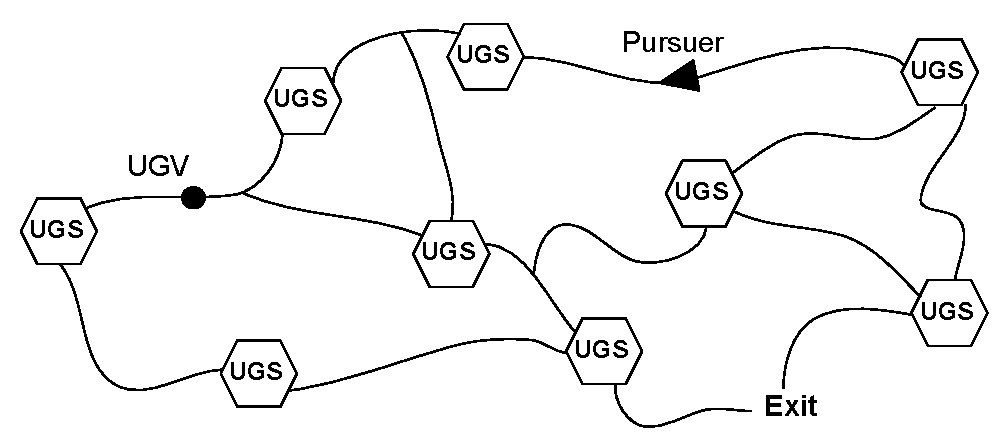
\includegraphics[width=0.35\textwidth]{Figures/RoadNet}
    	\caption{UGV in road network evading pursuer with information from noisy UGS.} 
        \label{fig:RoadNet}
        \vspace{-0.2cm}
    \end{figure}

\subsubsection{VIP Escort Example Application} \label{sec:vip_escort}
Consider a concrete grounding example problem based on the ``VIP escort'' scenario~\cite{Humphrey2012-lr}, which %can be viewed as a variant of the ``Minotaur's Labyrinth'' and 
serves as a useful proxy for security and surveillance applications with unmanned robotic vehicles (see Fig.~\ref{fig:RoadNet}). An unmanned ground vehicle (UGV) leads a small convoy protecting a VIP through a road network monitored by friendly unattended ground sensors (UGS). The road network also contains a hostile pursuer that the UGV is trying to evade while exiting the network as quickly as possible. The pursuer's location is unknown but can be estimated using intermittent data from the UGS, which only sense portions of the network and can produce false alarms. The UGV's decision space involves selecting a sequence of discrete actions (i.e. go straight, turn left, turn right, go back, stay in place). The UGS data, UGV motion, and pursuer behavior are all stochastic, and the problems of decision making and sensing are strongly coupled: some trajectories through the network allow the UGV to localize the pursuer before heading to the exit but incur a high time penalty); other trajectories afford rapid exit with high pursuer location uncertainty but increase the risk of getting caught by the pursuer, which can take multiple paths. A human supervisor monitors the UGV during operation. The supervisor does not have detailed knowledge of the UGV -- but can interrogate its actions, as well as potentially modify its decision making stance (`aggressively pursue exit' vs. `be very conservative and cautious') %and provide extra information about the pursuer (which is sporadically observed and follows an unknown course). 
in order better cope with the pursuer (which is sporadically observed and follows an unknown course). 

The physical states describing the combined motion of the UGV (whose states are always perfectly observable) and pursuer can be discretized in time and space to produce a Markov process model defined by some initial joint state probability distribution and joint state transition matrix, which depends on the steering actions taken by the UGV. The probability of obtaining `detection' and `no detection' data from each UGS given the true state of the pursuer can be modeled and used to update probabilistic beliefs about the state of the chaser. Finally, a reward function $R(x_k,u_k) = R_k$ can be specified for each time step $k$ to encode user preferences over the combined state of the UGV and pursuer, e.g. $R_k = -1$ for each time step the UGV is not co-located with the pursuer but not yet at the exit, $R_k= -1000$ if the UGV and pursuer are co-located, and $R_k=+1000$ if the UGV reaches the exit without getting caught. Given these elements, the UGV's navigational planning and decision-making problem may be generally formulated as a POMDP. %(more precisely: a mixed observability MDP, if the UGV states are always perfectly known). 
In special the case where the pursuer's state is fully observable at each step $k$ (e.g. due to very reliable and accurate UGS that cover all areas of the road network), the problem reduces to an MDP. 

%\nisar{add in more formal math notation...assume STM, obs model, rewards, etc...}

%\nisar{TODO: edit this: use some more formal MDP/POMDP notation...remove/compress bits at end...}One way to construct an autonomous UGV path planner is to discretize time and spatial variables to build a partially observable Markov decision process (POMDP) model \cite{Kochenderfer2015-uu} of the navigation task. The ideal POMDP solution is an optimal UGV action selection policy that will, \emph{on average}, maximize some utility function whose optimum value coincides with desirable UGV behaviors (i.e. avoiding the pursuer and exiting quickly). POMDP policies can be calculated by any number of sophisticated approximations that operate on probability distributions for the unknown pursuer state, which in turn can be found via Bayesian sensor fusion \cite{Ahmed2017-ph}. This defines at least two AIA capabilities per Fig.~\ref{fig:AIcapabilities}: knowledge representation and planning \footnote{consideration of lower-level UGV state estimation and control also leads to perception and motor control/execution.}. The trust-cycle terms here can then be defined as follows relative to the supervisor (user): \textit{AIA:} the combined POMDP planning and data fusion agent, which must make decisions under uncertainty; \textit{Trust:} the supervisor's willingness to rely on the UGV's planning and data fusion algorithms when the safety of the VIP being escorted is at stake; \textit{TRBs:} supervisor's behaviors that indicate trust (or lack thereof) in the UGV's planner; these include approving/rejecting the planner's actions, or real-time adjustments of the data fusion output based on what the supervisor receives from other intelligence sources; \textit{Assurances:} properties and behaviors of the planning agent that effect the supervisor's trust, e.g. communication of the escape success probability, reports that unexpected UGS data have been registered, or explanations of actions taken.
